%%%%%%%%%%%%%%%%%%%%%%%%%%%%%%%%%%%%%%%%%%%%%%%%%%%%%%%%%%
\section{previousWork}
\label{sec:previousWork}
%%%%%%%%%%%%%%%%%%%%%%%%%%%%%%%%%%%%%%%%%%%%%%%%%%%%%%%%%%
%\begin{figure}
%   {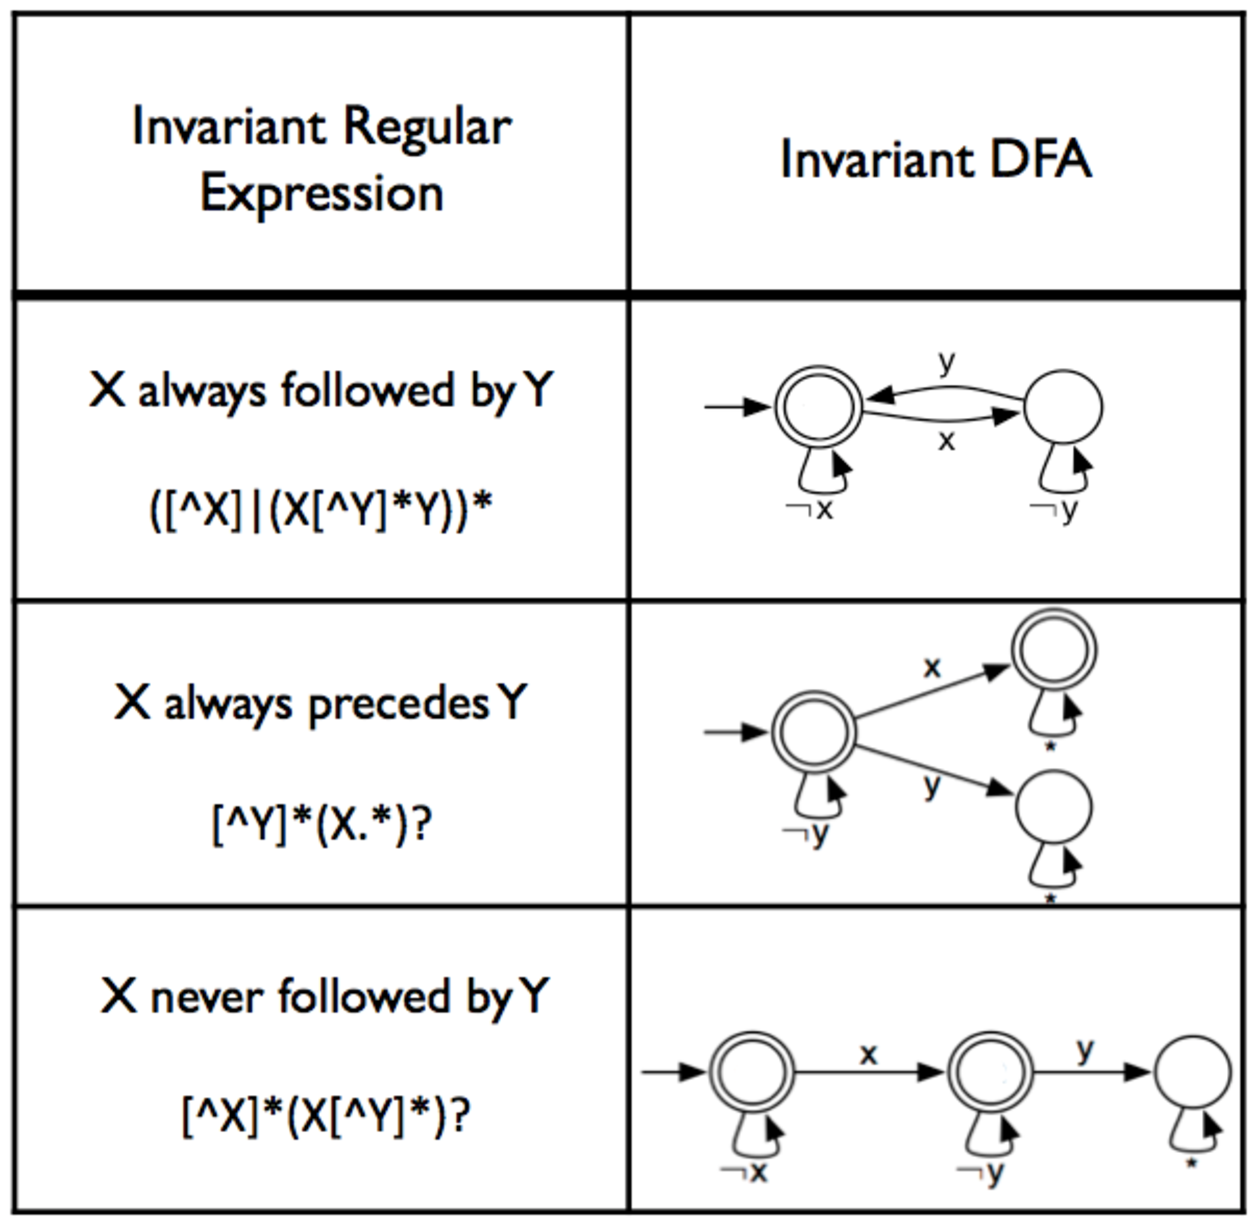
\includegraphics[width=\columnwidth]{fig/invRegexDfa.pdf}}
%   \caption{The regular expressions used to translate each invariant type into
%   an
%   invariant DFA.
%    } 
%   \label{fig:invRegDfa}
%\end{figure}
Previous work on this task has almost entirely been rule-based. The current state of the art approaches use a combination of regular-expression matching and hand-written interpretation functions to ground temporal expressions. These hand-built approaches are very domain-specific; they have a difficult time when applied to domains other than the one they were built for. Moreover, the complexities of natural language are often lost on these systems. Nested or hierarchical expressions are easy to handle when taking a parsing approach designed to deal with these phenomena, but these types of phrases can cause more rigid rule-based systems to fail. For example, phrases such as \emph{the third Wednesday of each month} or \emph{the second month of last year} are easier to ground using a parsing approach. 
While most of the work in this area has been on deterministic systems, one notable exception is ParsingTime~\cite{ParsingTime}. This system learned to parse from temporal phrases to logical forms, but is limited in that it doesn't take context into account. Their system uses a PCFG to parse the phrases to a logical form, then executes the form to get a result. However, their approach only looks at the temporal phrase itsef; it doesn't have any signal from the context in which the phrase appeared, such as verb tense or the result of parsing previously uttered phrases.

This work builds upon previous work using CCG for semantic parsing. 
